%link to template: https://www.overleaf.com/project/6593225db1459fc90d7950d0

\documentclass[10pt]{article}
\usepackage[spanish]{babel}
\usepackage[utf8]{inputenc}
\usepackage[OT1]{fontenc}
\usepackage{amsfonts, amsmath, amsthm, amssymb}
\usepackage{graphicx}
\usepackage{listings}
\usepackage[margin=1in]{geometry}
\usepackage{xcolor}
\newcounter{countCode}
\lstnewenvironment{code} [1][caption=Ponme caption, label=default]{%
	\renewcommand*{\lstlistingname}{Listado} 
	\setcounter{lstlisting}{\value{countCode}} 
	\lstset{ %
	language=java,
	basicstyle=\ttfamily\footnotesize,       % the size of the fonts that are used for the code
	numbers=left,                   % where to put the line-numbers
	numberstyle=\sc,      % the size of the fonts that are used for the line-numbers
	stepnumber=1,                   % the step between two line-numbers. 
	numbersep=5pt,                 % how far the line-numbers are from the code
	numberstyle=\color{red!50!blue},
    	backgroundcolor=\color{lightgray!20},
	rulecolor=\color{blue},
	keywordstyle=\color{red}\bfseries,
	showspaces=false,               % show spaces adding particular underscores
	showstringspaces=false,         % underline spaces within strings
	showtabs=false,                 % show tabs within strings adding particular underscores
	frame=single,                   % adds a frame around the code
	framexleftmargin=0mm,
	numberblanklines=false,
	xleftmargin=5pt,
	breaklines=true,
	breakatwhitespace=true,
	breakautoindent=true,
	captionpos=t,
	texcl=true,
	tabsize=2,                      % sets default tabsize to 3 spaces
	extendedchars=true,
	inputencoding=utf8, 
	escapechar=\%,
	morekeywords={print, println, size, background, strokeWeight, fill, line, rect, ellipse, triangle, arc, save, PI, HALF_PI, QUARTER_PI, TAU, TWO_PI, width, height,},
	emph=[1]{print,println,}, emphstyle=[1]{\color{blue}}, % Mis palabras clave.
	emph=[2]{width,height,}, emphstyle=[2]{\bf\color{violet}}, % Mis palabras clave.
	emph=[3]{PI, HALF_PI, QUARTER_PI, TAU, TWO_PI}, emphstyle=[3]\color{orange!50!violet}, % Mis palabras clave.
	emph=[4]{line, rect, ellipse, triangle, arc,}, emphstyle=[4]\color{green!70!black}, % Mis palabras clave.
	%emph=[5]{size, background, strokeWeight, fill,}, emphstyle=[5]{\tt \color{red!30!blue}}, % Mis palabras clave.
	%emph={[2]sqrt,baset}, emphstyle={[2]\color{blue}}, % f(sqrt(2)), sqrt a nivel 2 se pondrá azul
	#1}}{\addtocounter{countCode}{1}}



\title{Matrices}
\author{Victoria Hernández Yepes}
\date{\today}
\begin{document}
\maketitle \tableofcontents 


\begin{abstract}
En este documento se explican qué son las matrices, los distintos tipos que hay, algunas operaciones que se hacen con ellas con ellas (y sus respectivas propiedades), además de enseñar cómo realizar estas operaciones en programación. Incluye el concepto de relación binaria, y se explica cómo se pueden representar éstas (si son homogéneas) mediante grafos. y los distintos tipos de éstos últimos. Se recalca la ''matriz jacobiana'', explicando su función escalar y vectorial
\end{abstract}

\section{Definiciones}
En matemáticas, una matriz es todo conjunto de números o expresiones dispuestos en forma \textbf{rectangular}, formando filas y columnas. Una matriz se representa por medio de una letra mayúscula( A, B. ...).

\begin{equation}
\textbf{A} = \left[
\begin{array}{cccc}
a_{11} & a_{12} & \cdots & a_{1m} \\
a_{21} & a_{22} & \cdots & a_{2m} \\
\vdots & \vdots & \ddots & \vdots \\
a_{n1} & a_{n2} & \cdots & a_{nm} \\
\end{array}
\right]
\end{equation}

\begin{itemize}
 \item Cada uno de los números de que consta la matriz se denomina \textbf{elemento}. Un elemento se distingue de otro por la posición que ocupa, es decir, la fila y la columna a la que pertenece. Para ello se usa un doble subíndice donde el primero indica la fila y el segundo la columna a la que pertenece.
 
 Una forma simplificada de representar una matriz es $A:= ((a_{ij}))$
 \item El número de filas y columnas de una matriz se denomina \textbf{dimensión de una matriz}. A una matriz con n filas y m columnas se le denomina matriz n-por-m (escrito $n\times{m}$) donde n, m $\in{\mathbb{N}} - \{0\}$.
 \item Si la matriz tiene el mismo número de filas que de columnas, y es $n$, se dice que es de \textbf{orden} $n$.
 \item Dos matrices son \textbf{iguales} cuando tienen la misma dimensión y los elementos que ocupan el mismo lugar en ambas, son iguales.
 \item El conjunto de las matrices de tamaño $n \times{m}$ se representa como $\mathcal{M}_{n\times {m}}(\mathbb{K})$ donde $\mathbb{K}$ es el campo al cual pertenecen las entradas. El tamaño de una matriz siempre se da con el número de filas primero y el número de columnas después.
 \end {itemize}
 
\section{Tipos de Matrices}

\noindent\textbf{Matriz fila:} Una matriz fila está constituida por una sola fila.

\[\begin{bmatrix}
a_{11} & a_{12} & \cdots & a_{1m} \\
\end{bmatrix}\]

\noindent\textbf{Matriz columna:} La matriz columna tiene una sola columna.

\[\begin{bmatrix}
a_{11} \\
a_{21} \\
\vdots \\
a_{n1} \\
\end{bmatrix}\]

\textbf{Matriz rectangular:} La matriz rectangular tiene distinto número de filas que de columnas, siendo su dimensión $n\times {m}$. (Ver expresión (1)).

\textbf{Matriz traspuesta:} Dada una matriz $A$, se llama matriz traspuesta de A a la matriz que se obtiene cambiando ordenadamente las filas por las columnas y se denota por $A^t$.

Si A = (($a_{ij}$)), entonces $A^t$ = (($a_{ji}$))

Cumplen las siguiente propiedades:

\begin{itemize}
\item $(A^t)^t = A$.
\item $(A + B)^t = A^t + B^t$.
\item $(\alpha \cdot )^t = \alpha \cdot {A^t}$
\item $(A\times B)^t = B^t\times A^t$.
\end{itemize}
Las operaciones con matrices se definen en el apartado 3. \\


\textbf{Matriz nula:} En una matriz nula todos los elementos son ceros. $A = ((a_{ij})) = ((0))$ \\

\textbf{Matriz cuadrada:} La matriz cuadrada tiene el mismo número de filas que de columnas.

\begin{itemize}
\item Los elementos de la forma $((a_{ii}))$ constituyen \textbf{la diagonal principal}.
\item La \textbf{diagonal secundaria} la forman los elementos con $i + j = n + 1$, siendo $n$ el orden de la matriz.
\item Existen los siguientes tipos de matrices cuadradas\footnote{Las operaciones con matrices se definen en el apartado 3.}

\textit{Matriz triangular superior:} En una matriz triangular superior los elementos situados por debajo de la diagonal principal son ceros.

$$\textbf{A=}\begin{bmatrix}
a_{11} & a_{12} & \cdots & a_{1m} \\
0 & a_{22} & \cdots & a_{2m} \\
\vdots & \vdots & \ddots & \vdots \\
0 & 0 & \cdots & a_{nm}
\end{bmatrix}
$$

\textit{Matriz triangular inferior:} En una matriz triangular inferior los elementos situados por encima de la diagonal principal son ceros.

$$\textbf{A=}\begin{bmatrix}
a_{11} & 0 & \cdots & 0 \\
a_{21} & a_{22} & \cdots & 0 \\
\vdots & \vdots & \ddots & \vdots \\
a_{n1} & a_{n2} & \cdots & a_{nm}
\end{bmatrix}
$$

\textit{Matriz diagonal:} En una matriz diagonal todos los elementos que no están situados en la diagonal principal son nulos.

$$\textbf{A=}\begin{bmatrix}
a_{11} & 0 & \cdots & 0 \\
0 & a_{22}  & \cdots & 0 \\
\vdots & \vdots & \ddots & \vdots \\
0 & 0 & \cdots & a_{nm}
\end{bmatrix}
$$

\textit{Matriz escalar:} Una matriz  escalar es una matriz diagonal en la que los elementos de la diagonal principal son iguales.

\textit{Matriz identidad o unidad:} Una matriz  identidad es una matriz diagonal en la que los elementos de la diagonal principal son iguales a 1.

\textit{Matriz regular:} Una matriz  regular es una matriz cuadrada que tiene inversa.

\textit{Matriz singular:} Una matriz  singular no tiene matriz inversa.

\textit{Matriz indempotente:} Una matriz, $A$, es indempotente si: $A^2 = A$.

\textit{Matriz involutiva:} Una matriz, $A$, es involutiva si: $A^2 = I$.

\textit{Matriz simétrica:} Una matriz simétrica es una matriz cuadrada que verifica: $A = A^t$.
\textit{Matriz antisimétrica o hemisimétrica:} Una matriz antisimétrica o hermisimétrica es una matriz cuadrada que verifica $A = -A^t$.

\textit{Matriz ortogonal:} Una matriz es ortogonal si verifica que: $A\times {A^t} = I$

\end{itemize}

\section{Operaciones con Matrices}
Las operaciones que se pueden hacer con matrices provienen de sus aplicaciones, sobre todo de las aplicaciones en álgebra lineal. De ese modo las operaciones, o su forma muy particular de ser implementadas, no son únicas.

\subsection{Suma o adición}

\noindent \textbf{Definición}

Se define la operación de suma o adición de matrices como una operación binaria
$$
+ : \mathcal{M}_{n\times {m}}(\mathbb{K})\times {\mathcal{M}_{n\times {m}}(\mathbb{K})} \rightarrow \mathcal{M}_{n\times {m}}(\mathbb{K})
$$
tal que $(A, B) \longmapsto C = A+B$ y donde $c_{ij} = a_{ij} + b_{ij}$ en el que la operación de suma en la última expresión es la operación binaria correspondiente pero en el campo $\mathbb{K}$. \\

\noindent \textbf{Ejemplo}

Sea $A, B \in \mathcal{M_3}(\mathbb{R})$

$$
\begin{bmatrix}
1 & 3 & 2 \\
1 & 0 & 0 \\
1 & 2 & 2 \\
\end{bmatrix}
+
\begin{bmatrix}
1 & 0 & 5 \\
7 & 5 & 0 \\
2 & 1 & 1 \\
\end{bmatrix}
=
\begin{bmatrix}
1+1 & 3+0 & 2+5 \\
1+7 & 0+5 & 0+0 \\
1+2 & 2+1 & 2+1 \\
\end{bmatrix}
=
\begin{bmatrix}
2 & 3 & 7 \\
8 & 5 & 0 \\
3 & 3 & 3 \\
\end{bmatrix}
$$

La entrada $c_{12}$ es igual a la suma de los elementos $a_{12}$ y $b_{12}$ lo cual es $a_{12} + b_{12}$. \\

\noindent\textbf{Propiedades}

\begin{itemize}
\item \textit{Asociatividad:} $( A + B) + C = A + (B + C)$
\item \textit{Conmutatividad:} $(A + B) = (B + A)$
\item \textit{Existencia del elemento neutro aditivo:} Existe $0\in \mathcal{M}_{n\times {m}}(\mathbb{K})$ tal que $A + 0 = 0 + A = A$
\item \textit{Existencia del inverso aditivo:} Existe $D\in \mathcal{M}_{n\times {m}}(\mathbb{K})$ tal que $A + D = 0$ a esta matriz $D$ se le denota por $-A$
\end{itemize}

\noindent\textbf{Estructura algebraica}

La operación binaria adición se dice que esta operación es una operación interna por lo que se cumple intrínsecamente la propiedad de que $\mathcal{M}_{n\times {m}}(\mathbb{K})$ es cerrado bajo adición. Con estas propiedades se tiene que $(\mathcal{M}_{n\times {m}}(\mathbb{K}), + )$ es un grupo abeliano.

En el caso en que el conjunto al que pertenecen las entradas de la matriz sea un anillo $(A, +_A, \cdot{_A})$, la operación de adición de matrices continúa dotando de estructura de grupo abeliano a $(\mathcal{M}_{n\times {m}}(A), +)$, ya que bajo un anillo $(A, +_A, \cdot{_A})$ se tiene que $(A, +_A)$ es un grupo abeliano. En el caso de que las entradas estén en un grupo $(G, +_G)$, éste necesita ser un grupo abeliano para que la adición de matrices siga dotando de estructura de grupo abeliano a $(\mathcal{M}_{n\times {m}}(G), +)$ \\


\noindent\textbf{Programación} \\

En psuedocódigo basado en Java, esta operación es:
\begin{code}[caption=Suma de Matrices, label=default]
void main() {
  float [][] a = creaMatriz(n, m); // Capturamos los valores de la matriz A \\
  float [][] b = creaMatriz(n, m); // Capturamos los valores de la matriz A \\
  float [][] suma = suma (a, b); ; // Invocamos a la función que suma matrices. \\
} 

// La suma de dos matrices es otra matriz
float [][] suma(float[][] matriz1, float [][] matriz2) {
   // Si no hay matrices no hay nada que hacer.
   if (matriz1 ==null || matriz2==null) return null;
   
   // Asumimos que el primer índice es la fila y el segundo es la columna.
   // El número de filas y columnas en ambas matrices tienen que ser iguales.
   if (matriz1.length != matriz2.length) return null; // Filas diferentes.
   else
     for (int i=0; 1<matriz1.length; i++) {
       if (matriz1[0].length != matriz1[i].length) 
         return null; // Alguna fila tiene un número diferente de columnas
         
       if (matriz1[i].length != matriz2[i].length)
         return null; //  matrices tienen columnas diferentes.
     }
   // Ya estamos en condiciones de empezar
   
   // Primero creamos la nueva matriz
   // Tiene tantas filas y columnas, como la primera (o segunda) matriz.
   float [][] sol = new float[matriz1.length][matriz1[0].length];
   
   // Completamos las celdillas de la nueva matriz con el típico bucle anidado.
   for (int i=0; i<sol.length; i++)
     for (int j=o; j<sol[i].length; j++)
     
       sol[i][j] = matriz1[i][j]+matriz2[i][j]; // En esta celdilla calcularemos la suma.
   return sol;
}    
\end{code}

\subsection{Producto por un escalar}

\noindent\textbf{Definición}

Sea $A \in (\mathcal{M}_{n\times {m}}(\mathbb{K})$ y $\lambda \in \mathbb{K}$. Se define la operación de producto por un escalar como una función  
$$
\cdot : \mathbb{K} \times \mathcal{M}_{n\times {m}}(\mathbb{K}) \longrightarrow \mathcal{M}_{n\times {m}}(\mathbb{K})
$$
tal que $(\lambda, A) \mapsto B = \lambda A$ y donde $b_{ij} = \lambda a_{ij}$ en donde el producto es la operación binaria correspondiente pero en el campo $\mathbb{K}$ \\

\noindent\textbf{Ejemplo} 

Sea $A \in \mathcal{M}_{2\times {3}}(\mathbb{R})$ y $2 \in \mathbb{R}$
$$
2
\begin{bmatrix}
1 & 8 & -3 \\
4 & -2 & 6 \\
\end{bmatrix}
=
\begin{bmatrix}
2(1) & 2(8) & 2(-3) \\
2(4) & 2(-2) & 2(6) \\
\end{bmatrix}
=
\begin{bmatrix}
2 & 16 & -6 \\
8 & -4 & 12 \\
\end{bmatrix}
$$

Por ejemplo, la entrada $b_{12}$ es igual al producto $\lambda a_{12}$. \\

\noindent\textbf{Propiedades}


Sean $A,B \in (\mathcal{M}_{n\times {m}}(\mathbb{K})$ y $\lambda, \mu \in \mathbb{K}$, donde $\mathbb{K}$ es un campo, entonces se cumplen las siguientes propiedades para la operación producto por un escalar

\begin{itemize}
\item \textit{Asociatividad:} $(\lambda \mu)A = \lambda(\mu A)$
\item \textit{Distribuitividad respecto de la suma de matrices:} $\lambda(A+B) = \lambda A + \lambda B$
\item \textit{Distribuitividad respecto de la suma en el campo:} $(\lambda + \mu)A = \lambda A + \mu A$
\item \textit{Producto por el neutro multiplicativo del campo:} $1_{\mathbb{K}}A = A$
\end{itemize}

\noindent\textbf{Estructura algebráica}


Por como se definió la operación de producto por escalares se dice que $\mathcal{M}_{n\times {m}}(\mathbb{K})$ es cerrado bajo producto por escalares. Con estas propiedades y las de la adición se tiene que $\mathcal{M}_{n\times {m}}(\mathbb{K})$ es un espacio vectorial con las operaciones de suma y producto por escalares definidas antes.

En el caso de que las entradas y los escalares no estén en un campo sino en un anillo entonces no necesariamente existe el neutro multiplicativo. En caso de que exista, con lo cual el anillo es un anillo con uno, se dice que $\mathcal{M}_{n\times {m}}(A)$ es un módulo sobre $A$. \\

\noindent\textbf{Programación} \\

En psuedocódigo basado en Java, esta operación es:

\begin{code}[caption=Suma de Matrices, label=default]
void main() {
  float [][] a = creaMatriz(n, m); // Capturamos los valores de la matriz A \\
  float L = leeCte; // Capturamos el valor de la constante. \\
  float [][] sol = productoEscalarMatriz (L, a); // Calculamos el producto. \\
} 

// La suma de dos matrices es otra matriz
float [][] suma(float lambda, float[][] matriz) {
   // Si no hay matrices no hay nada que hacer.
   if (matriz1 ==null) return null;
   
   // Primero creamos la nueva matriz
   // Tiene tantas filas y columnas, como la primera (o segunda) matriz.
   float [][] sol = new float[matriz.length][matriz[0].length];
   
   // Completamos las celdillas de la nueva matriz con el típico bucle anidado.
   for (int i=0; i<sol.length; i++)
     for (int j=o; j<sol[i].length; j++)
     
       sol[i][j] = lambda * matriz[i][j]; // En esta celdilla calcularemos el producto
       
   return sol;
}    
\end{code}
\subsection{Producto Matricial}

Su definición depende del contexto. Cuando proviene de la composición de aplicaciones lineales el tamaño de la matriz corresponde con las dimensiones de los espacios vectoriales entre los cuales se establece la aplicación lineal. De ese modo el producto de matrices representa la composición de aplicaciones lineales.

En efecto, en ciertas bases tenemos que $f : V \longrightarrow W$ se puede representar como $f(x) = Ax$ donde $x$ es la representación de un vector de $V$ en la base que se ha elegido para $V$ en forma de vector columna. Si tenemos dos aplicaciones lineales $f : V \longrightarrow W$ y $g : W \longrightarrow U$ entonces $f(x) = g(f(x)) = g(Bx) = AB(x)$ donde $AB$ es el producto de las representaciones matriciales de $f, g$. Nótese que la composición no se puede dar entre cualquier aplicación sino entre aplicaciones que vaya de $V \rightarrow W \rightarrow U$, en particular debe de haber una relación entre las dimensiones de los espaciones vectoriales. Una vez dicho esto podemos definir el producto de la siguiente manera. \\

\noindent\textbf{Definición}

Sean $A \in \mathcal{M}_{n\times {m}}(K)$ y  $B \in \mathcal{M}_{m\times {p}}(K)$. Se define el producto de matrices como una función
$$
\cdot : \mathcal{M}_{n\times {m}}(K) \times \mathcal{M}_{m\times {p}}(K) \longrightarrow \mathcal{M}_{n\times {p}}(K)
$$ 
tal que $(A,B) \mapsto C = AB$ y donde $c_{ij}= \sum\limits_{k=1}^m a_{ik}b_{kj}$ para toda $i, j$, es decir
$$
c_{ij} = a_{i1}b_{1j} + a_{i2}b_{2j} + a_{i3}b_{3j} + \ldots + a_{im}b_{mj}
$$ \\

\noindent\textbf{Ejemplo}

Sean $A \in \mathcal{M}_{2\times {3}}(R)$ y $B \in \mathcal{M}_{3\times {2}}(R)$:
$$
\begin{bmatrix}
2 & 0 & -2 \\
-1 & 3 & 1 \\
\end{bmatrix}
\begin{bmatrix}
3 & 1 \\
2 & 1 \\
1 & 0 \\
\end{bmatrix}
=
\begin{bmatrix}
1(3) + 0(2) + 2(1) & 1(1) + 0(1) + 2(0) \\
-1(3) + 3(2) + 1(1) & -1(1) + 3(1) + 1(0) \\
\end{bmatrix}
=
\begin{bmatrix}
5 & 1 \\
4 & 2 \\
\end{bmatrix}
$$
donde la matriz es como habíamos establecido en la definición: una matriz $C in \mathcal{M}_{2\times {2}}(R)$. Por ejemplo, la entrada $c_{12} = a_{11}b_{12} + a_{12}b_{22} + a_{13}b_{32} + \ldots + a_{1m}b_{m2}$ \\

\noindent\textbf{Propiedades}

\begin{itemize}
\item \textit{Asociatividad:} $A(BC) = (AB)C$
\item \textit{Distribuitividad respecto de la suma de matrices por la izquierda:} $A(B+C) = AB + AC$
\end{itemize}


\noindent\textbf{Estructura algebraica}

El producto de matrices no es conmutativo, si lo fuera la composición de funciones lineales sería conmutativa y eso en general no sucede. Obviamente existen casos particulares de algunos tipos de matrices en los que sí hay conmutatividad. En el caso de que tengamos $\mathcal{M}_n(\mathbb{K})$ tendremos que el producto entre matrices en $\mathcal{M}_n(\mathbb{K})$ también está en $\mathcal{M}_n(\mathbb{K})$. En ese caso, $\mathcal{M}_n(\mathbb{K})$ además de espacio vectorial es un álgebra sobre un campo. En el caso de que el conjunto al que pertenecen las entradas sea un anillo conmutativo con uno, entonces $\mathcal{M}_n(A)$ además de módulo es un álgebra sobre un anillo. Más aún $(\mathcal{M}_n(\mathbb{K}), +, \cdot)$ con $\cdot$ el producto de matrices es un anillo. \\

\noindent\textbf{Programación} \\

En psuedocódigo basado en Java, esta operación es:

\begin{code}[caption=Suma de Matrices, label=default]
void main() {
  float [][] a = creaMatriz(n, m); // Capturamos los valores de la matriz A \\
  float [][] b = creaMatriz(m, k); // Capturamos los valores de la matriz B \\
  float [][] sol = producto (a, b);  // Calculamos el producto \\
} 

// El producto de dos matrices es otra matriz
float [][] producto (float[][] matriz1, float[][] matriz2) {
   // Si no hay matrices no hay nada que hacer.
   if (matriz1==null || matriz2==null) return null;
   
   // Asumimos que el primer índice es la fila y el segundo es la columna.
   // El número de columnas de la primera tienen que ser igual al número
   // de filas de la primera.
   if (matriz1[0].length != matriz2.length) return null;
   
   // Aquí habría que poner el código para comprobar que todos los vectores
   // tienen la misma longitud. Ver el código de cómo sumar (ahí está desarrollado).
   
   // Ya estamos en condiciones de empezar
   
   // Primero creamos la nueva matriz
   // Tiene tantas filas, como filas tiene la primera.
   //Tiene tantas columnas, como columnas tiene la segunda.
   // Asumimos que matriz2[i]==matriz2[0]
   float [][] sol = new float[matriz1.length][matriz2[0].length];
   
   // Completamos las celdillas de la nueva matriz con el típico bucle anidado.
   for (int i=0; i<sol.length; i++)
     for (int j=o; j<sol[i].length; j++) {
       // En esta celdilla calcularemos una suma, así que inicializamos a cero.
       sol[i][j] = 0;
       
       // Hacemos tantas sumas como números de columnas tiene la primera.
       // Para los índices (i, j), recorremos la fila i de la primera
       // y la columna j de la segunda.
       for (int k=0; k<matriz1[i].length; k++) {
         sol[i][j] += matriz1[i][k] * matriz2[k][j];
       }
     }
     
   return sol;
}    
\end{code}

\section{Matrices Binarias y Grafos} 


\subsection{Relaciones binarias}

En matemáticas, una relación binaria es una relación matemática $\mathcal{R}$ definida entre los elementos de dos conjuntos $A$ y $B$. Una relación $\mathcal{R}$ de $A$ en $B$ se puede representar mediante pares ordenador $8a,b)$ para los cuales se cumple una propiedad $\mathcal{P}(a,b)$, de forma que $(a,b) \in A\times B$, y se anota:

$$
\mathcal{R} = \{(a,b) \in A\times B  \mid   \mathcal{P}(a,b)\}
$$

Que se lee: la relación binaria $\mathcal{R}$ es el conjunto de pares ordenados $(a,b)$ pertenecientes al producto cartesiano $a\times B$, y para los cuales se cumple la propiedad $\mathcal{P}$ que los relaciona.

Las propiedades siguientes son correctas para representar la relación binaria $\mathcal{R}$ entre los elementos $a$ y $b$:

$$
a\mathcal{R}b \hspace{1cm} o \hspace{1cm}\mathcal{R}(a,b)\hspace{1cm} o\hspace{0.2cm}bien\hspace{1cm}(a,b) \in \mathcal{R}
$$

Una relación binaria homogénea es la que se da entre los elementos de un único conjunto, llamando $A$ al conjunto, tendríamos: $R(a,b) : (a,b) \in A^2$.

También podemos representar una relación binaria homogénea como una correspondencia de $A$ sobre $A: R: A \rightarrow A$

Tomando como conjunto inicial al conjunto $A$ y como final también al conjunto $A$, nos permite asociar un elemento incial a otro final dentro de un mismo conjunto, determinando una operación matemática o función de cálculo y no una estructura interna, teniendo siempre en cuenta, que si bien el conjunto inicial y final son un mismo conjunto, la relación es unidireccional, y si el elemento $a$ está relacionado con el $b$ no implica, necesariamente, que el $b$ li esté con el $a$.


\subsection{Grafos}

Las relaciones binarias homogéneas se pueden representar mediante grafos.

En matemáticas y ciencias de la computación, un grafo (del griego grafo: dibujo, imagen) es un conjunto de objetos llamados vértices o nodos unidos por enlaces llamados aristas o arcos, que permiten representar relaciones binarias entre elementos de un conjunto o un objeto de estudio dela teoría de grafos. Típicamente, un grafo se representa gráficamente como un conjunto de punto (vértices o nodos) unidos por líneas (aristas).


Desde un punto de vista práctico, los grafos nos permiten estudiar las interrelaciones entre unidades que interactúan unas con otras. Por ejemplo, una red de computadoras puede representarse y estudiarse mediante un grafo, en el cual los vértices representan terminales y las aristas representan conexiones (las cuales, a su vez, pueden ser cables o conexiones inalámbricas).

Un grafo $G$ es un par ordenado $G = (V,E)$, donde :

\begin{itemize}
\item $V$ es un conjunto de vértices o nodos, y
\item E es un conjunto de aristas o arcos, que relacionan estos nodos.
\end{itemize}


Normalmente $V$ suele ser finito. Muchos resultados importantes sobre grafos no son aplicables para grados infinitos.

\begin{itemize}
\item Se llama orden del grafo $G$ a su número de vértices, .
\item El grado de un vértice o nodo $v \in V$ es igual al número de arcos que lo tienen como extremo.
\end{itemize}

\noindent\textbf{Tipos de Grafos}

Los grafos pueden ser dirigidos, no dirigidos o mixtos.

\begin{itemize}
\item Un grafo dirigido o digrafo es un grafo $G = (V,E)$ donde:
\begin{itemize}
\item $V\not= \emptyset$
\item $E \subseteq \{(a,b) \in V\times V \colon a \not= b\}$ es un conjunto de pares ordenados de elementos de $V$.
\end{itemize}
Dada una arista $(a,b)$, $a$ es un nodo inicial y $b$ su nodo final.

Un ejemplo es la Figura 2. \\
\begin{center}
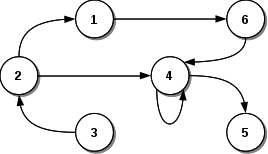
\includegraphics[width=0.3\textwidth]{grafodirigido} \\
Figura 1: . Un ejemplo de grafo dirigido
\end{center} 






\item Un grafo no dirigido es un grafo $G = (V,E)$ donde:
\begin{itemize}
\item $V\not= \emptyset$
\item $E \subseteq \{x \in \mathcal{P}(V) \colon |x|=2\}$ es un conjunto de pares ordenados de elementos de $V$.
\end{itemize}
\end{itemize}
Un par no ordenado es un conjunto de la forma $(a,b)$, de manera que $(a,b)=(b,a)$. Para los grafos, estos conjuntos pertenecen al conjunto potencia de $V$, denotado $\mathcal{P}(V)$, y son de cardinalidad $2$.

Un ejemplo es la figura 2. \\
\begin{center}
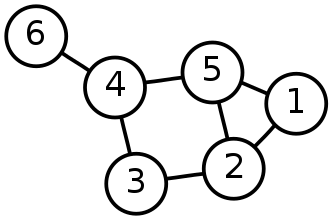
\includegraphics[width=0.3\textwidth]{grafo} \\
Figura 2: . Un ejemplo de grafo no dirigido
\end{center}

\begin{itemize}
\item Un grafo mixto es aquel que se define con la capacidad de poder contener aristas dirigidas y no dirigidas. Tano los grafos dirigidos como los no dirigidos son casos particulares de este.
\end{itemize}


\subsection{Representación de grafos}

Una matriz lógica, matriz binaria, matriz de relación, matriz booleana o matriz $(0,1)$, es una matriz con entradas del dominio booleano $B = 0, 1$. Tal matriz puede ser usada para representar una relación binaria entre un par de conjuntos finitos y en particular a los grafos.

Las dos representaciones principales de grafos son las siguientes: \\

\noindent\textbf{Matriz de adyacencia (MA):}  Se utiliza una matriz de tamaño $n\times m$ donde las filas y las columnas hacen referencia a los vértices para almacenar en cada casilla la longitud entre cada par de vértices del grafo. La celda $M [i,j]$ almacena la longitud entre el vértice $i$ y el vértice $j$. Si su valor es infinito significa que no existe arista entre esos vértices, y y $M A[i,j] = 0$. \\
\begin{center}
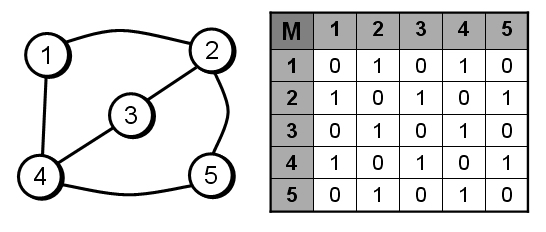
\includegraphics[width=0.5\textwidth]{Matrizdeadyacencia} \\
Figura 3: . Un ejemplo de matriz de adyacencia
\end{center}



En pseudocódigo basado en Java, para construir la matriz de adyacencia de la Figura 3 es:

\begin{code}[caption=Matriz de Adyacencia, label=default]
boolean [][] grafo = new int[5][5]; // Grafo sobre 5 elementos.

for (int i=0; i < grafo.length; i++)
  for (int j=o; j < grafo[i].length; j++)  {
    boolean hayUno = ((i0 || i== 4) && (j==1 || j==3)) ||
            ((i=1 || i== 3) && (j==0 || j==1 || j==4));
    
    if (hayUno) grafo[i][j]=1;
    else grafo[i][j] = 0;
   }
}   
\end{code}

\noindent\textbf{Lista de adyacencia (LA):} Se utiliza un vector de tamaño $n$ (un elemento por cada vértice) donde $LA[i]$ almacena la referencia a una lista de los vértices adyacentes a $i$. En una red esta lista almacenará también la longitud de la arista que va desde $i$ al vértice adyacente. \\
\begin{center}
\centering
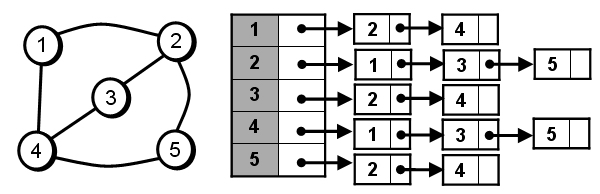
\includegraphics[width=0.6\textwidth]{Listasdeadyacencia} \\
Figura 3: . Un ejemplo de matriz de adyacencia
\end{center}


Podemos simular las listas mediante arrays con filas de longitud variable. En pseudocódigo basado en Java para la Figura 4 es:

\begin{code}[caption=Lista de Adyacencia con Arrays, label=default]
boolean [][] grafo = new int[5][]; // Grafo sobre 5 elementos.

for (int i=0; i < grafo.length; i++)
  if (i==0 || i ==2 || i==3) grafo[i] = new int[2];
  else grafo[i] = new int[3];
  
  for(int j=0; j < grafo[i].length; j++) {
    if (i mod 2 = 0) grafo[i][j] = 2*j + 2;
    else grafo[i][j] = 2*j + 1;
   }
}   
\end{code}

\section{Matriz Jacobiana}

En cálculo vectorial, se llama jacobiano o determinante jacobiano al determinante de la matriz jacobiana. Tanto la matriz jacobiana como el determinante jacobiano reciben su nombre en honor al matemático Carl Gustav Jacobi.

La matriz jacobiana es una matriz formada por las derivadas parciales de primer orden de una función. Una de las aplicaciones más interesantes de esta matriz es la posibilidad de aproximar linealmente a la función en un punto. En este sentido, el jacobiano representa la derivada de una función multivariable. Propiamente  deberíamos  hablar  más  que  de  matriz  jacobiana,  de  diferencial  jacobiana  o  aplicación lineal  jacobiana  ya  que  la  forma  de  la  matriz  dependerá de  la  base  o  coordenadas  elegidas.  Es  decir, dadas  dos  bases  diferentes  la  aplicación  lineal  jacobiana  tendrá  componentes  diferentes  aún  tratándose del  mismo  objeto  matemático.  La  propiedad  básica  de  la  ”matriz”jacobiana  es  la  siguiente,  dada  una aplicación  cualquiera $\mathbf{F} \colon \mathbb{R}^n \rightarrow \mathbb{R}^m$ continua, es decir $\mathbf{F} \in \mathcal{C}^k(\mathbb{R}^N,\mathbb{R}^m)$ se dirá que es diferenciable si existe una aplicación lineal $\lambda \in \mathcal{L}(\mathbb{R}^n,\mathbb{R}^m)$ tal que:
\begin{equation}
\lim\limits_{||x-y|| \to 0}\frac{||\mathbf{F(x) - F(y) y \lambda(x-y)||}}{\mathbf{||x-y||}}=0
\end{equation}

Una  de  las  aplicaciones  más  interesantes  de  esta  matriz  es  la  posibilidad  de  aproximar  linealmente a  la  función  en  un  punto.  También  se  aplica  en  modelado  cinemático  de  un  robot.  En  dicho  modelado se busca las relaciones entre las variables articulares y la posición (expresada normalmente en forma de coordenadas  cartesianas)  y  orientación  del  extremo  del  robot.  En  esta  relación  no  se  tienen  en  cuenta las fuerzas o pares que actúan sobre el robot (actuadores, cargas, fricciones, etc.) y que pueden originar el movimiento del mismo. La matriz jacobiana directa permite conocer las velocidades del extremo del robot  a  partir  de  los  valores  de  las  velocidades  de  cada  articulación.  Por  su  parte,  la  matriz  Jacobiana inversa permitirá conocer las velocidades determinadas en el extremo del robot.

\subsection{Función escalar}

Empecemos con el caso más sencillo de una función escalar $F \colon \mathbb{R}^n \rightarrow \mathbb{R}$. En  este  caso  la  matriz jacobiana será una matriz formada por un vector fila que coincide con el gradiente. Si la función admite derivadas parciales para cada variable puede verse que basta definir la ”matriz”jacobiana como:

\begin{equation*}
\mathbf{\lambda(x)} := \mathbf{\nabla}F(x) = \frac{\partial F(x)}{\partial x_1} \ldots \frac{\partial F(x)}{\partial x_n}
\end{equation*}

Ya que entonces se cumplirá la relación (2) automáticamente, por lo que en este caso la "matriz jacobiana" es precisamente el gradiente.

\subsection{Función vectorial}

Supongamos $\mathbf{F} \colon \mathbb{R}^n \rightarrow \mathbb{R}^m$ es una función que va del espacio euclídeo $n$-dimensional a otro espacio $m$-dimensional. Esta función está determinada por $m$ funciones escalares reales:

\begin{equation*}
y_i = F_i(x_1, \ldots, x_n), \hspace{1.2cm} \mathbf{y=F(x)=}(F_1(x),\ldots,F_m(x))
\end{equation*}

Cuando la función anterior es diferenciable, entonces las derivadas parciales de estas $m$ funciones pueden ser organizadas en una matriz $m$ por $n$, la matriz jacobiana de $F$:

$$
\begin{bmatrix}
\frac{\partial y_1}{\partial x_1} & \cdots & \frac{\partial y_1}{\partial x_n} \\
\vdots & \ddots & \vdots \\
\frac{\partial y_m}{\partial x_1} & \cdots & \frac{\partial y_m}{\partial x_n}
\end{bmatrix}
$$

Esta matriz es notada de diversas maneras:

$$
\mathcal{J}_\textbf{F}(x_1, \ldots, x_n),\hspace{0.8cm} o \hspace{0.8cm} \frac{\partial(y_1,\ldots, y_m)}{\partial(x_1,\ldots, x_n)},\hspace{0.8cm} o \hspace{0.8cm} D\textbf{F}(x_1, \ldots, x_n),\hspace{0.8cm} o \hspace{0.8cm} \mathbf{\nabla F}(x_1, \ldots, x_n) 
$$

Nótese que la fila $i$-ésima fila coincidirá dada con el gradiente de la función $yi$, para $i=1,\ldots,m$.

Si $p$ es un punto de $R^n$ y $F$ es diferenciable en $p$, entonces su derivada está dada por $JF(p)$. En este caso, la aplicación lineal descrita por $JF(p)$ es la mejor aproximación lineal de $F$ cerca del punto $p$, de esta manera:

$$
\mathbf{F(x) \approx F(p) + J_F(p)(x-p)}
$$

para $x$ cerca de $p$. O con mayor precisión:

$$
\lim\limits_{||x-p|| \to 0}\frac{||\mathbf{F(x) - F(p) -J_F(p)(x-p)||}}{\mathbf{||x-p||}}=0
$$


En ciertos espacios vectoriales de dimensión no finita, formados por funciones, puede generalizarse el conccepto de matriz jacobiana definiendo una aplicación lineal jacobiana.

\subsection{Ejemplos}

\noindent\textbf{Ejemplo 1.} La matriz jacobiana de la función $F \colon R^3 \rightarrow R^3$ definida como:

$$
F(x_1, x_2, x_3) = (x_1, 5x_3, 4x_2^2 - 2x_3)
$$

viene dada por

$$
J_F(x_1, x_2, x_3) =
\begin{bmatrix}
1 & 0 & 0 \\
0 & 0 & 5 \\
0 & 8x_2 & -2
\end{bmatrix}
$$


\noindent\textbf{Ejemplo 2.} No siempre la matriz jacobiana es cuadrada, como en el siguiente ejemplo.


Supóngase la función $F \colon R^3 \rightarrow R^4$, cuyas componentes son:

$$
y_1 = 1/x_1
y_2 = 5x_3
y_3 = 4x_2^2 - 2x_3
y_4 = x_3sin(x_1)
$$

Aplicando la definición de matriz jacobiana:

\begin{equation*}
J_F(x_1, x_2, x_3) = 
{\LARGE\begin{bmatrix}
\frac{\partial y_1}{\partial x_1} & \frac{\partial y_1}{\partial x_2} & \frac{\partial y_1}{\partial x_3} \\
\frac{\partial y_2}{\partial x_1} & \frac{\partial y_2}{\partial x_2} & \frac{\partial y_2}{\partial x_3} \\
\frac{\partial y_3}{\partial x_1} & \frac{\partial y_3}{\partial x_2} & \frac{\partial y_3}{\partial x_3} \\
\frac{\partial y_4}{\partial x_1} & \frac{\partial y_4}{\partial x_2} & \frac{\partial y_4}{\partial x_3} 
\end{bmatrix}}
=
\begin{bmatrix}
-1/x_1^2 & 0 & 0 \\
0 & 0 & 5 \\
0 & 8x_2 & -2 \\
x_3cos(x_1) & 0 & sin(x_1)
\end{bmatrix}
\end{equation*}

\section{Maxima}
\end{document}

